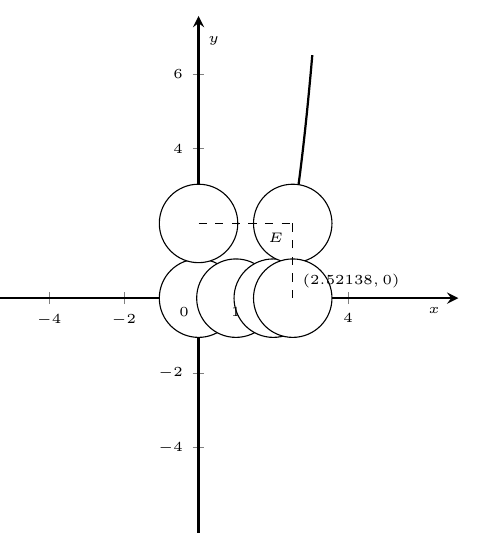
\begin{tikzpicture}
\begin{axis}[ 
xlabel=$x$,
ylabel=$y$,
axis x line=center, xlabel style={anchor=north west},
axis y line=center, ylabel style={anchor=south west},
xmin=-4.5,
xmax=5.9,
ymin=-5.5,
ymax=6.5,
axis line style={thick, shorten > = -0.5cm, shorten < = -0.5cm},
samples=50,
unit vector ratio*=1 1,
font=\tiny
]
\addplot [domain=0:5.099, thick, black, smooth]{x*(x-1)*(x-2)};
  \coordinate (A) at (axis cs:0,0) {};
\coordinate (B) at (axis cs:1,0) {};
\coordinate (C) at (axis cs:2,0) {};
\coordinate (D) at (axis cs:0,2) {};
\draw [fill= white] (A) circle [radius=1.05];
\draw [fill= white] (B) circle [radius=1.05];
\draw [fill= white] (C) circle [radius=1.05];
\draw [fill= white] (D) circle [radius=1.05];
\node[below left] at (A) {$0$};
\node[below ] at (B) {$1$};
%\node[below right] at (C) {$2$};
%\node[below left] at (D) {$C$};
\coordinate (E) at (axis cs:2.52138,2) {}; 
\draw [fill= white] (E) circle [radius=1.05];
\node[below left] at (E) {$E$};
\draw[dashed] (D)--(E);
\coordinate (F) at (axis cs:2.52138,0) {}; 
\draw [fill= white] (F) circle [radius=1.05];
\node[above right] at (F) {$(2.52138,0)$};
\draw[dashed] (F)--(E);
 \end{axis};
\end{tikzpicture}